% generated by Plantuml 1.2024.3       
\definecolor{plantucolor0000}{RGB}{255,255,255}
\definecolor{plantucolor0001}{RGB}{24,24,24}
\definecolor{plantucolor0002}{RGB}{0,0,0}
\definecolor{plantucolor0003}{RGB}{226,226,240}
\definecolor{plantucolor0004}{RGB}{254,255,221}
\definecolor{plantucolor0005}{RGB}{238,238,238}

\begin{adjustbox}{width=.9\paperwidth, center}
	\resizebox{\textwidth}{!}{
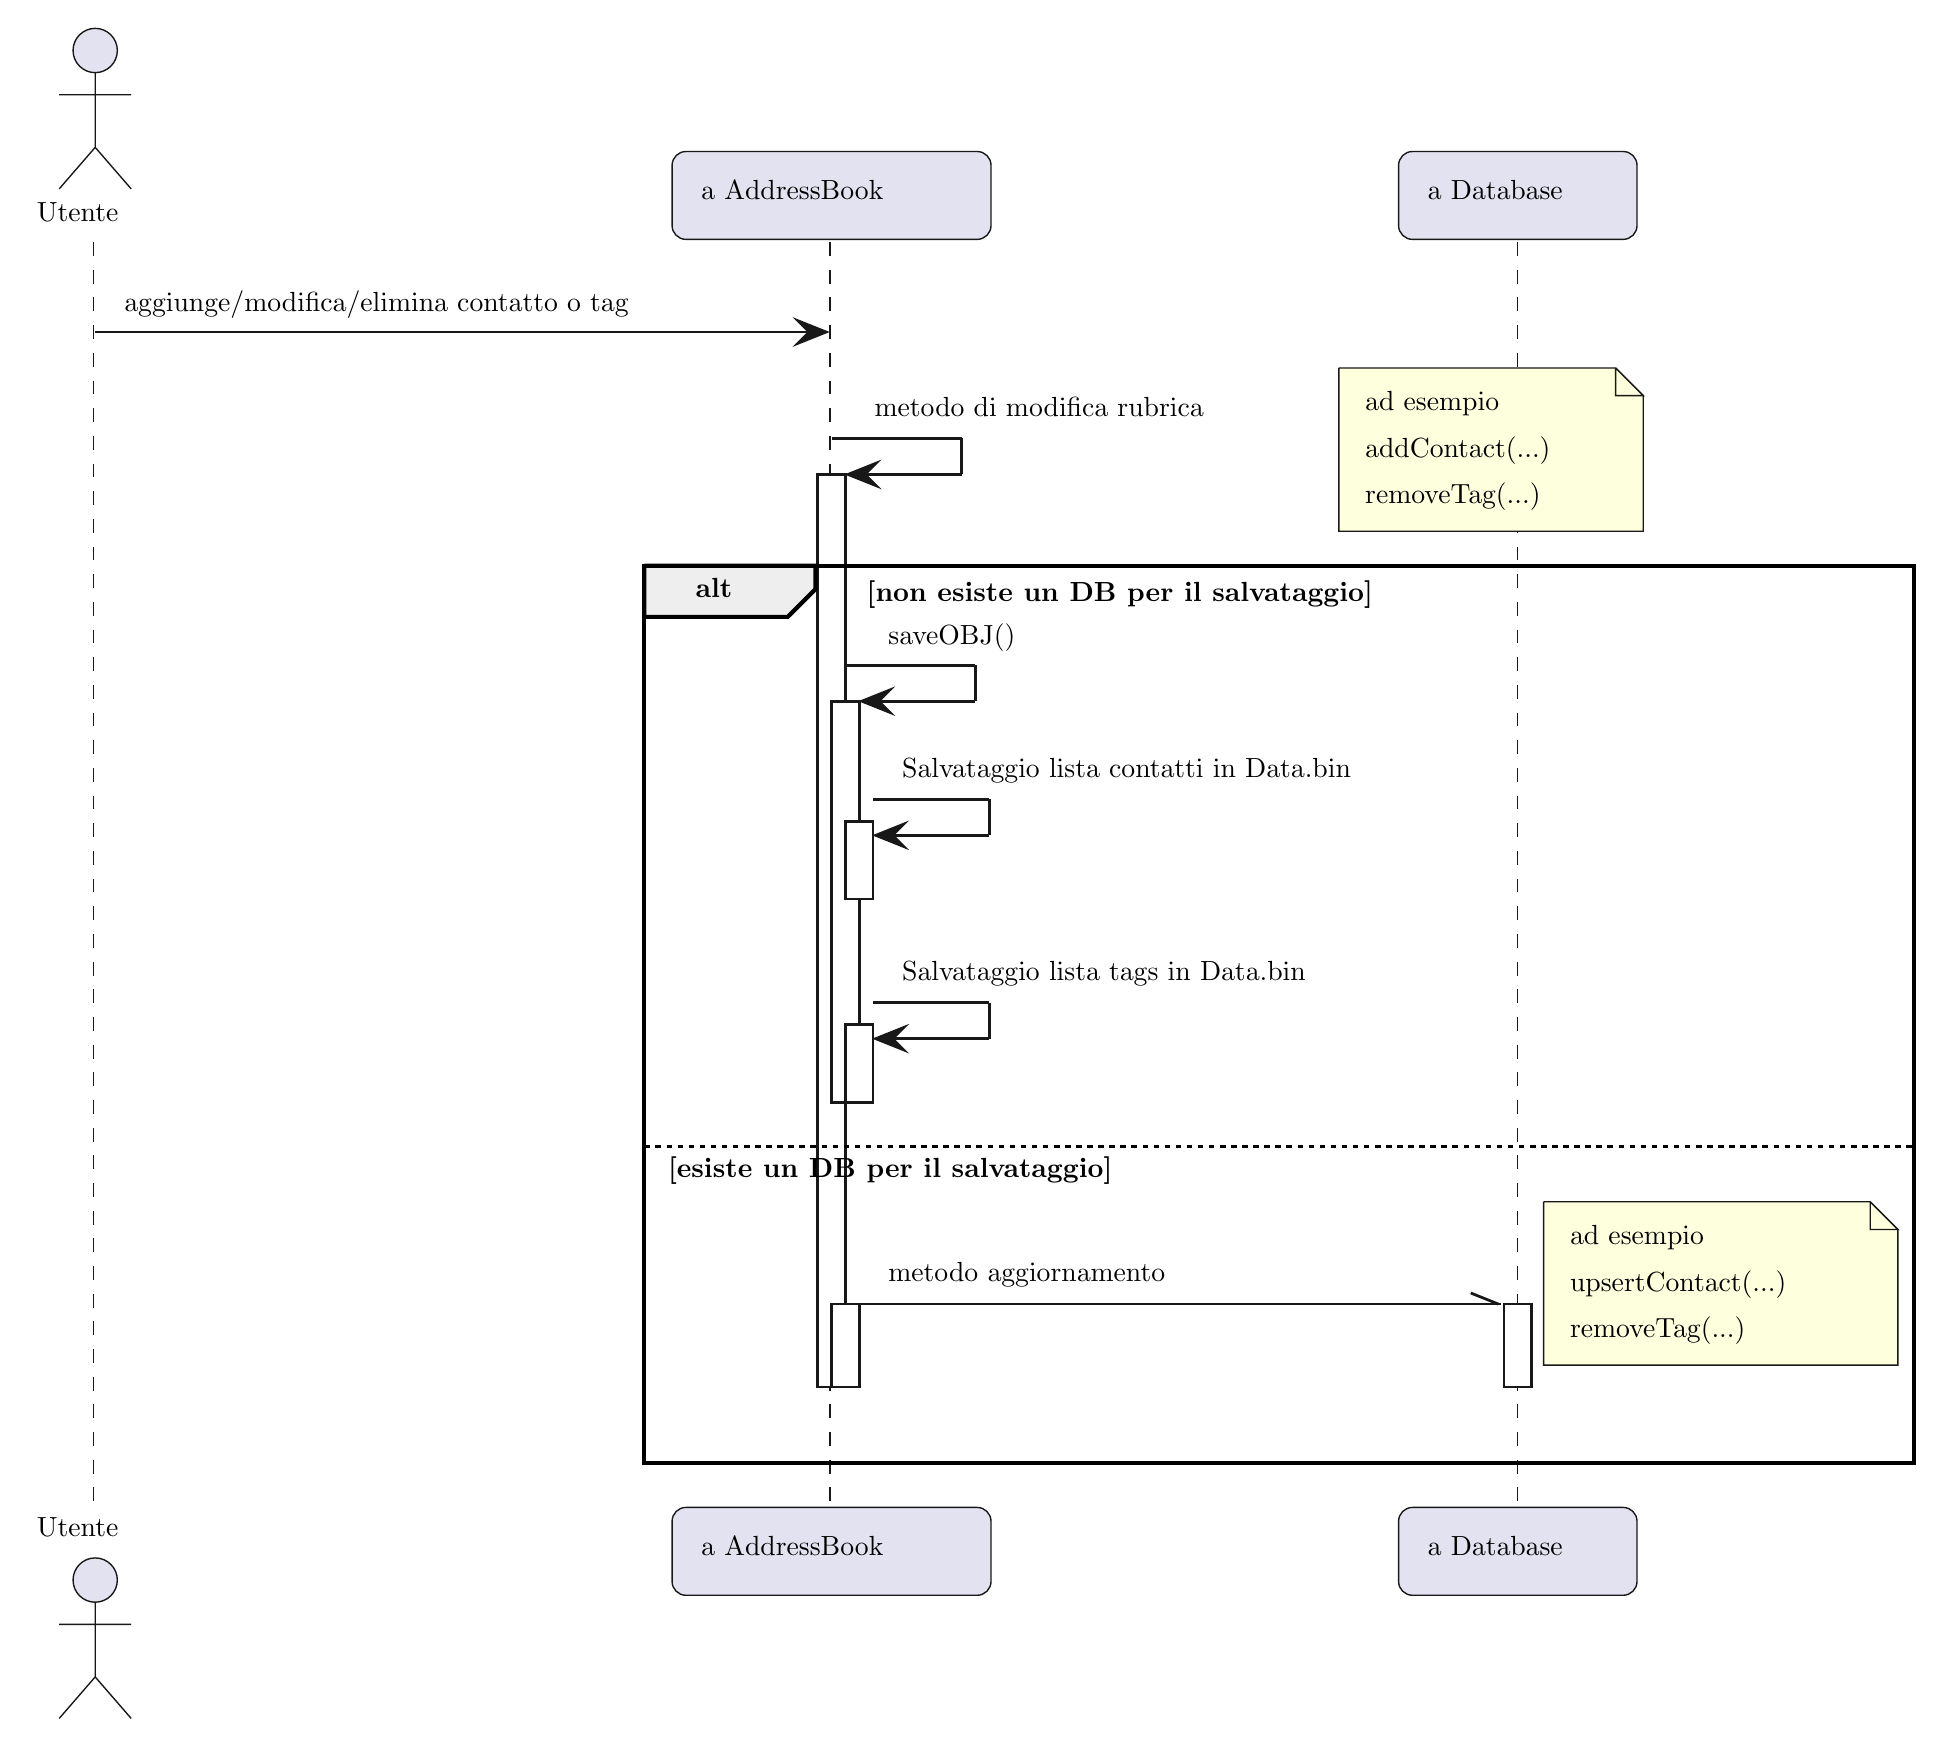
\begin{tikzpicture}[yscale=-1
,pstyle0/.style={color=plantucolor0001,fill=white,line width=1.0pt}
,pstyle1/.style={color=black,line width=1.5pt}
,pstyle2/.style={color=plantucolor0001,line width=0.5pt,dash pattern=on 5.0pt off 5.0pt}
,pstyle3/.style={color=plantucolor0001,fill=plantucolor0003,line width=0.5pt}
,pstyle4/.style={color=plantucolor0001,line width=0.5pt}
,pstyle5/.style={color=plantucolor0001,fill=plantucolor0001,line width=1.0pt}
,pstyle6/.style={color=plantucolor0001,line width=1.0pt}
,pstyle7/.style={color=plantucolor0001,fill=plantucolor0004,line width=0.5pt}
]
\draw[pstyle0] (290.6771pt,166.6816pt) rectangle (300.6771pt,496.4746pt);
\draw[pstyle0] (295.6771pt,248.6172pt) rectangle (305.6771pt,393.5742pt);
\draw[pstyle0] (300.6771pt,292.0957pt) rectangle (310.6771pt,320.0957pt);
\draw[pstyle0] (300.6771pt,365.5742pt) rectangle (310.6771pt,393.5742pt);
\draw[pstyle0] (295.6771pt,466.4746pt) rectangle (305.6771pt,496.4746pt);
\draw[pstyle0] (538.6553pt,466.4746pt) rectangle (548.6553pt,496.4746pt);
\draw[pstyle1] (228.0535pt,199.6602pt) rectangle (686.7392pt,523.9531pt);
\draw[pstyle2] (29pt,82.7461pt) -- (29pt,540.9531pt);
\draw[pstyle2] (295.0535pt,82.7461pt) -- (295.0535pt,540.9531pt);
\draw[pstyle2] (543.5799pt,82.7461pt) -- (543.5799pt,540.9531pt);
\node at (5pt,65pt)[below right,color=black]{Utente};
\draw[pstyle3] (29.6pt,13.5pt) ellipse (8pt and 8pt);
\draw[pstyle4] (29.6pt,21.5pt) -- (29.6pt,48.5pt)(16.6pt,29.5pt) -- (42.6pt,29.5pt)(29.6pt,48.5pt) -- (16.6pt,63.5pt)(29.6pt,48.5pt) -- (42.6pt,63.5pt);
\node at (5pt,539.9531pt)[below right,color=black]{Utente};
\draw[pstyle3] (29.6pt,566.1992pt) ellipse (8pt and 8pt);
\draw[pstyle4] (29.6pt,574.1992pt) -- (29.6pt,601.1992pt)(16.6pt,582.1992pt) -- (42.6pt,582.1992pt)(29.6pt,601.1992pt) -- (16.6pt,616.1992pt)(29.6pt,601.1992pt) -- (42.6pt,616.1992pt);
\draw[pstyle3] (238.0535pt,55pt) arc (180:270:5pt) -- (243.0535pt,50pt) -- (348.3006pt,50pt) arc (270:360:5pt) -- (353.3006pt,55pt) -- (353.3006pt,76.7461pt) arc (0:90:5pt) -- (348.3006pt,81.7461pt) -- (243.0535pt,81.7461pt) arc (90:180:5pt) -- (238.0535pt,76.7461pt) -- cycle;
\node at (245.0535pt,57pt)[below right,color=black]{a AddressBook};
\draw[pstyle3] (238.0535pt,544.9531pt) arc (180:270:5pt) -- (243.0535pt,539.9531pt) -- (348.3006pt,539.9531pt) arc (270:360:5pt) -- (353.3006pt,544.9531pt) -- (353.3006pt,566.6992pt) arc (0:90:5pt) -- (348.3006pt,571.6992pt) -- (243.0535pt,571.6992pt) arc (90:180:5pt) -- (238.0535pt,566.6992pt) -- cycle;
\node at (245.0535pt,546.9531pt)[below right,color=black]{a AddressBook};
\draw[pstyle3] (500.5799pt,55pt) arc (180:270:5pt) -- (505.5799pt,50pt) -- (581.7307pt,50pt) arc (270:360:5pt) -- (586.7307pt,55pt) -- (586.7307pt,76.7461pt) arc (0:90:5pt) -- (581.7307pt,81.7461pt) -- (505.5799pt,81.7461pt) arc (90:180:5pt) -- (500.5799pt,76.7461pt) -- cycle;
\node at (507.5799pt,57pt)[below right,color=black]{a Database};
\draw[pstyle3] (500.5799pt,544.9531pt) arc (180:270:5pt) -- (505.5799pt,539.9531pt) -- (581.7307pt,539.9531pt) arc (270:360:5pt) -- (586.7307pt,544.9531pt) -- (586.7307pt,566.6992pt) arc (0:90:5pt) -- (581.7307pt,571.6992pt) -- (505.5799pt,571.6992pt) arc (90:180:5pt) -- (500.5799pt,566.6992pt) -- cycle;
\node at (507.5799pt,546.9531pt)[below right,color=black]{a Database};
\draw[pstyle0] (290.6771pt,166.6816pt) rectangle (300.6771pt,496.4746pt);
\draw[pstyle0] (295.6771pt,248.6172pt) rectangle (305.6771pt,393.5742pt);
\draw[pstyle0] (300.6771pt,292.0957pt) rectangle (310.6771pt,320.0957pt);
\draw[pstyle0] (300.6771pt,365.5742pt) rectangle (310.6771pt,393.5742pt);
\draw[pstyle0] (295.6771pt,466.4746pt) rectangle (305.6771pt,496.4746pt);
\draw[pstyle0] (538.6553pt,466.4746pt) rectangle (548.6553pt,496.4746pt);
\draw[pstyle5] (283.6771pt,111.2246pt) -- (293.6771pt,115.2246pt) -- (283.6771pt,119.2246pt) -- (287.6771pt,115.2246pt) -- cycle;
\draw[pstyle6] (29.6pt,115.2246pt) -- (289.6771pt,115.2246pt);
\node at (36.6pt,96.7461pt)[below right,color=black]{aggiunge/modifica/elimina contatto o tag};
\draw[pstyle6] (295.6771pt,153.6816pt) -- (342.6771pt,153.6816pt);
\draw[pstyle6] (342.6771pt,153.6816pt) -- (342.6771pt,166.6816pt);
\draw[pstyle6] (301.6771pt,166.6816pt) -- (342.6771pt,166.6816pt);
\draw[pstyle5] (311.6771pt,162.6816pt) -- (301.6771pt,166.6816pt) -- (311.6771pt,170.6816pt) -- (307.6771pt,166.6816pt) -- cycle;
\node at (307.6771pt,135.2031pt)[below right,color=black]{metodo di modifica rubrica};
\draw[pstyle7] (478.9801pt,128.2246pt) -- (478.9801pt,187.2246pt) -- (588.9801pt,187.2246pt) -- (588.9801pt,138.2246pt) -- (578.9801pt,128.2246pt) -- (478.9801pt,128.2246pt);
\draw[pstyle7] (578.9801pt,128.2246pt) -- (578.9801pt,138.2246pt) -- (588.9801pt,138.2246pt) -- (578.9801pt,128.2246pt);
\node at (484.9801pt,133.2246pt)[below right,color=black]{ad esempio};
\node at (484.9801pt,149.7031pt)[below right,color=black]{addContact(...)};
\node at (484.9801pt,166.1816pt)[below right,color=black]{removeTag(...)};
\draw[color=black,fill=plantucolor0005,line width=1.5pt] (228.0535pt,199.6602pt) -- (289.8535pt,199.6602pt) -- (289.8535pt,208.1387pt) -- (279.8535pt,218.1387pt) -- (228.0535pt,218.1387pt) -- (228.0535pt,199.6602pt);
\draw[pstyle1] (228.0535pt,199.6602pt) rectangle (686.7392pt,523.9531pt);
\node at (243.0535pt,200.6602pt)[below right,color=black]{\textbf{alt}};
\node at (304.8535pt,201.6602pt)[below right,color=black]{\textbf{[non esiste un DB per il salvataggio]}};
\draw[pstyle6] (300.6771pt,235.6172pt) -- (347.6771pt,235.6172pt);
\draw[pstyle6] (347.6771pt,235.6172pt) -- (347.6771pt,248.6172pt);
\draw[pstyle6] (306.6771pt,248.6172pt) -- (347.6771pt,248.6172pt);
\draw[pstyle5] (316.6771pt,244.6172pt) -- (306.6771pt,248.6172pt) -- (316.6771pt,252.6172pt) -- (312.6771pt,248.6172pt) -- cycle;
\node at (312.6771pt,217.1387pt)[below right,color=black]{saveOBJ()};
\draw[pstyle6] (310.6771pt,284.0957pt) -- (352.6771pt,284.0957pt);
\draw[pstyle6] (352.6771pt,284.0957pt) -- (352.6771pt,297.0957pt);
\draw[pstyle6] (311.6771pt,297.0957pt) -- (352.6771pt,297.0957pt);
\draw[pstyle5] (321.6771pt,293.0957pt) -- (311.6771pt,297.0957pt) -- (321.6771pt,301.0957pt) -- (317.6771pt,297.0957pt) -- cycle;
\node at (317.6771pt,265.6172pt)[below right,color=black]{Salvataggio lista contatti in Data.bin};
\draw[pstyle6] (310.6771pt,357.5742pt) -- (352.6771pt,357.5742pt);
\draw[pstyle6] (352.6771pt,357.5742pt) -- (352.6771pt,370.5742pt);
\draw[pstyle6] (311.6771pt,370.5742pt) -- (352.6771pt,370.5742pt);
\draw[pstyle5] (321.6771pt,366.5742pt) -- (311.6771pt,370.5742pt) -- (321.6771pt,374.5742pt) -- (317.6771pt,370.5742pt) -- cycle;
\node at (317.6771pt,339.0957pt)[below right,color=black]{Salvataggio lista tags in Data.bin};
\draw[color=black,line width=1.0pt,dash pattern=on 2.0pt off 2.0pt] (228.0535pt,409.5742pt) -- (686.7392pt,409.5742pt);
\node at (233.0535pt,409.5742pt)[below right,color=black]{\textbf{[esiste un DB per il salvataggio]}};
\draw[pstyle6] (536.6553pt,466.4746pt) -- (526.6553pt,462.4746pt);
\draw[pstyle6] (305.6771pt,466.4746pt) -- (537.6553pt,466.4746pt);
\node at (312.6771pt,447.9961pt)[below right,color=black]{metodo aggiornamento};
\draw[pstyle7] (553pt,429.5176pt) -- (553pt,488.5176pt) -- (681pt,488.5176pt) -- (681pt,439.5176pt) -- (671pt,429.5176pt) -- (553pt,429.5176pt);
\draw[pstyle7] (671pt,429.5176pt) -- (671pt,439.5176pt) -- (681pt,439.5176pt) -- (671pt,429.5176pt);
\node at (559pt,434.5176pt)[below right,color=black]{ad esempio};
\node at (559pt,450.9961pt)[below right,color=black]{upsertContact(...)};
\node at (559pt,467.4746pt)[below right,color=black]{removeTag(...)};
\end{tikzpicture}
}
\end{adjustbox}
